

%%%%%%%%%%%%%%%%%%%%% LateX template %%%%%%%%%%%%%%%%%


%%%%%%%%%%%% inicio del documento incluyendo opciones %%%%%%%%%%%%%%%%%%%%%%%%%%%%%%%
\documentclass[letterpaper,11pt]{article}
%%%%%%%%%%%%%%%%%%%%%%%%%%%%%%%%%%%%%%%%%%%%%%%%%%%%%%%%%%%%%%%%%%%%%%%%%%%%

%%%%%%% paquetes utiles: español, incluir graficos, etc %%%%%%%%%%%%%%%%%%%%%%%%%%%%
\usepackage[utf8]{inputenc}
\usepackage{amsmath}
\usepackage{amsfonts}
\usepackage{amssymb}
\usepackage{amsthm}
\usepackage[spanish]{babel}
\usepackage{latexsym}
\usepackage{euscript}
\usepackage{graphicx}
\usepackage{tdclock}
\usepackage{braket}
\usepackage[autostyle=true]{csquotes}
\usepackage{braket}
\usepackage{pdfpages}
\usepackage{subcaption} 
%%%%%%%%%%%%%%%%%%%%%%%%%%%%%%%%%%%%%%%%%%%%%%%%%%%%%%%%%%%%%%%%%%%%%%%%%%%%%%%%%%

%%%%%%%%%%%%%%%%%%% espacio para la primera linea del parrafo %%%%%%%%%%%%%%%
\setlength{\parindent}{0mm} 
%%%%%%%%%%%%%%%%%%%%%%%%%%%%%%%%%%%%%%%%%%%%%%%%%%%%%%%%%%%%%%%%%%%%%%%%%%

%%%%%%%%%%%%%%% espacio entre parrafos %%%%%%%%%%%%%%%%%%%%%%%%%%%%%%%
\setlength{\parskip}{2mm}
%%%%%%%%%%%%%%%%%%%%%%%%%%%%%%%%%%%%%%%%%%%%%%%%%%%%%%%%%%%%%%%%%%%%

%%%%%%%%%%%%%%%%%%%%% espaciado entre lineas %%%%%%%%%%%%%%%%%%%%%%%%%%%%%
\linespread{1} 
%%%%%%%%%%%%%%%%%%%%%%%%%%%%%%%%%%%%%%%%%%%%%%%%%%%%%%%%%%%%%%%%%%%%%%

\renewcommand{\vec}[1]{\mathbf{#1}}

%%%%%%%%%%%%%%%%%%%%%%%% Control de margenes %%%%%%%%%%%%%%%%%%%%%%%%%%%%
%\setlength{\topmargin}{-1.cm}
\setlength{\oddsidemargin}{-.8cm}
\setlength{\evensidemargin}{-.8cm}
\setlength{\textheight}{24cm} 
\setlength{\textwidth}{18cm} 
\setlength{\headsep}{-2cm}
%%%%%%%%%%%%%%%%%%%%%%%%%%%%%%%%%%%%%%%%%%%%%%%%%%%%%%%%%%%%%%%%%%%%%%%%%%%%

%%%%%%%%%%%%%%%  definicion de comandos que se utilicen frecuentemente %%%%%%%%%%%%%%%
\def\und#1{\underline{#1}}
\def\be{\begin{equation}}
\def\ee{\end{equation}}
\def\bea{\begin{eqnarray}}
\def\eea{\end{eqnarray}}
%%%%%%%%%%%%%%%%%%%%%%%%%%%%%%%%%%%%%%%%%%%%%%%%%%%%%%%%%%%%%%%%%%%%%%%%%%%%%%%%%%%%

%%%%%%%%%%% Aqui se inicia el contenido del documento %%%%%%%%%%%%%%%%%%%%%%%%%%%%%%%%
\begin{document}

\begin{center}
{\bf \Large Tiempo de retorno cuántico} 
\end{center}

\noindent
{\bf \large Nombre: Carlos Manuel Rodríguez Martínez} \hspace{5.2cm} {\bf \large Fecha: 25/10/2015} 

\smallskip

\section{Tiempo de retorno}
En el artículo \textit{Quantum revivals versus classical periodicity in the infinite square well} \cite{RT} se resuelve una aparente paradoja de incongruencia de los resultados que se obtienen en la mecánica cuántica respecto a la mecánica clásica.

Cuando una partícula de masa $M$ se encuentra en un pozo de potencial infinito se espera que su periodo de oscilación sea $T_{cl} = L \sqrt{\frac{2 M}{E}}$, donde $L$ es la longitud del pozo. Este periodo de oscilación se calcula fácilmente utilizando mecánica newtoniana. Este resultado no es el mismo (aparentemente) que el que se obtiene al calcular este tiempo utilizando la mecánica cuántica, donde
\[
	T_{rev} = \frac{4 M L^2}{\pi \hbar}.
\]
Este es el tiempo en que $\psi(x, 0) = \psi(x, T_{rev})$, donde $\psi$ es la función de onda que describe al estado cuántico.
Pero la función de onda no es una magnitud medible, en un experimento sólo se puede medir el valor esperado de una magnitud. Por ejemplo, si
\[
	\ket{\psi(t)} = \sum_{n=1}^\infty c_n e^{- \frac{i E_n t}{\hbar}} \ket{n},
\]
entonces
\[
	\braket{x(t)} = \braket{\psi(t) | x | \psi(t)} = \sum_{m \, \text{par}} \sum_{n \, \text{impar}} 2 \mathcal{R}e (c_m^* c_n e^{i(E_m - E_n) t /\hbar}) \braket{m | x | n}.
\]

Como $\braket{m | x | n}$ se anula para $m$ y $n$ con la misma paridad, entonces el valor esperado de la posición es una suma de términos de Fourier con periodos de
\[
	\frac{2 \pi}{E_m - E_n} = \frac{T_{rev}}{m^2 - n^2}.
\]

Para un estado inicial cuasi clásico, la energía de $n$ estados que van desde $n_C - r$ a $n_c + r$, donde $r << n_C$, y donde $i$, $j$ son enteros que van desde $-r$ a $+r$, para $i$ par y $j$ impar, los términos de Fourier tienen periodos
\[
	\frac{T_{rev}}{(n_C + i)^2 - (n_C + j)^2} = \frac{T_{rev}}{2 n_C (i-j) + i^2 - j^2} \approx \frac{T_{rev}}{2 n_C (i-j)}.
\]
Es decir, que los periodos son aproximadamente
\[
	\frac{T_{rev}}{2 n_C},\, \frac{T_{rev}}{2 n_C (3)},\, \frac{T_{rev}}{2 n_C (5)}, \cdots, \frac{T_{rev}}{2 n_C (2 r - 1)}.  
\]
Pero la suma de Fourier que representa el valor esperado de la posición tiene un periodo promedio de
\[
	T_{pos} = \frac{T_{rev}}{2 n_C}.
\]
Si se define la energía central correspondiente al eigenestado central
\[
	E_C = E_1 n_C^2,
\]
entonces el periodo de posición es
\[
	T_{pos} = \frac{T_{rev}}{2 \sqrt{E_C/E_1}} = \frac{\pi \hbar}{\sqrt{E_1 E_C}} .
\]
Sustituyendo $E_1$ queda
\[
	T_{pos} = L \sqrt{\frac{2 M}{E_C}},
\]
que es lo mismo que en el caso clásico. Así la paradoja queda resuelta.

\section{Comparación entre tiempos de retorno clásico y cuántico}
Se realizó una comparación entre los tiempos de retorno clásico y cuántico tomando la evolución temporal de un paquete de onda que corresponde al primer eigenestado del pozo de potencial infinito, con un momento $p$. Este paquete es de la forma
\[
	\psi (x,0) = \sqrt{\frac{2}{L}} \sin \left(\frac{\pi  x}{L}\right) e^{i k x}.
\]
Los eigenestados del pozo de potencial infinito son de la forma
\[
	\phi_n (x) = \sqrt{\frac{2}{L}} \sin \left(\frac{\pi  n x}{L}\right),
\]
y los eigenvalores de energía son
\[
	E_n = \frac{n^2 \pi ^2 \hbar^2}{2 M L^2}.
\]
Para obtener la evolución temporal se aplica el operator evolución al estado en el tiempo $t = 0$,
\[
	\psi (x,t) = \hat{U}(t) \psi (x,0) = e^{- \frac{i}{\hbar} \hat{H}} \psi (x,0).
\]
Para poder aplicar el operator de evolución conviene expresar la función de onda el términos de los eigenestados del hamiltoniano,
\[
	\psi (x,0) = \sum_{n = 0}^\infty c_n \phi_n(x).
\]
Los coeficientes se pueden obtener a través de la integración. Cómo estamos en un pozo de potencial infinito se pueden pasar los límites de integración de $\int_{-\infty}^\infty$ a $\int_0^L$,
\[
	c_n = \int_0^L \psi (x,0) \phi_n (x) \, dx.
\]
Así, la evolución temporal queda como
\[
	\psi (x,t) = \sum_{n = 0}^\infty c_n \phi_n (x) e^{- \frac{i}{\hbar} E_n t}.
\]

\begin{figure}[h!]
\centering
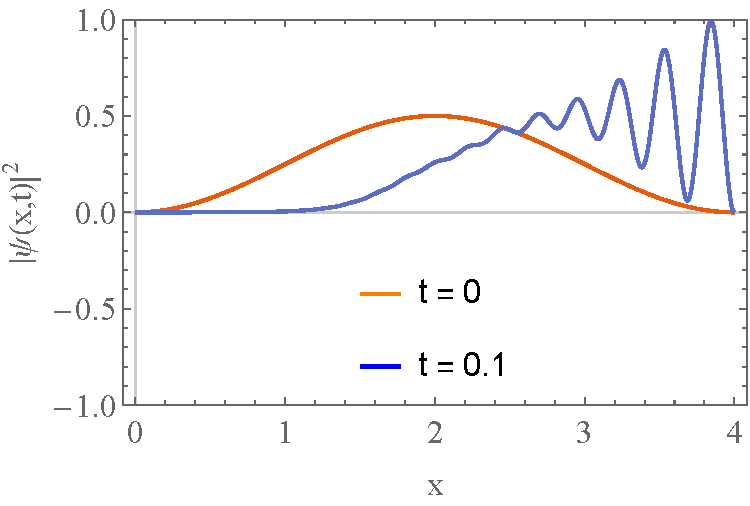
\includegraphics[scale=0.55]{img/rt_evol}
\caption{Evolución temporal de $\psi(x,t)$, $k = 10$.}
\label{fig:ev}
\end{figure}

En la implementación del código se pueden  hacer algunas consideraciones de el rango en el cual se debe hacer la sumatoria de $\psi (x,t)$. Esto depende de la energía del paquete inicial, la cual se codifica en el momento que se le da a la partícula. Para bajas energías dominan los primeros términos de $c_n$, mientras que conforme aumenta la energía los términos relevantes de $c_n$ son cada vez más altos (figura \ref{fig:cn}).

\begin{figure}[h!]
\centering
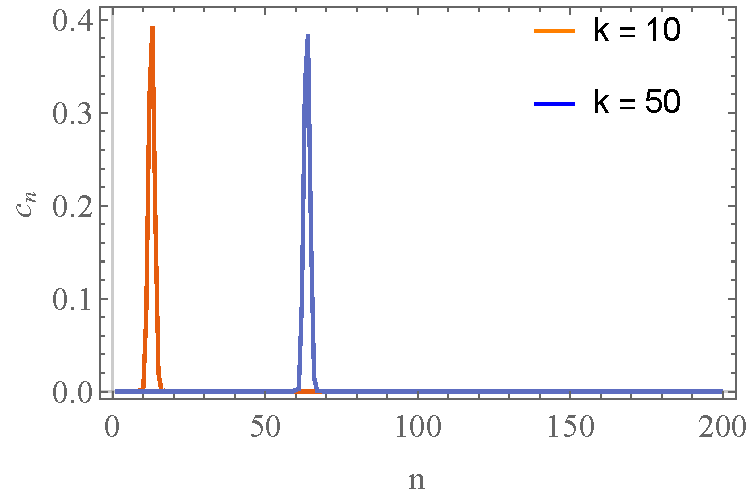
\includegraphics[scale=0.55]{img/rt_coef}
\caption{Valores de $c_n$ para diferentes energías.}
\label{fig:cn}
\end{figure}

Para asegurarnos de tomar suficientes valores de $c_n$ pedimos que se cumpla
\[
	\sum_{n = i}^j |c_n|^2 > 0.99.
\]

Para obtener el tiempo de retorno nos interesa medir el valor de expectación de la posición $\braket{\hat{x}}$, el cual se calcula mediante
\[
	\braket{\hat{x}(t)} = \int_0^L x |\psi(x,t)|^2 \, dx.
\]

\begin{figure}[h!]
\centering
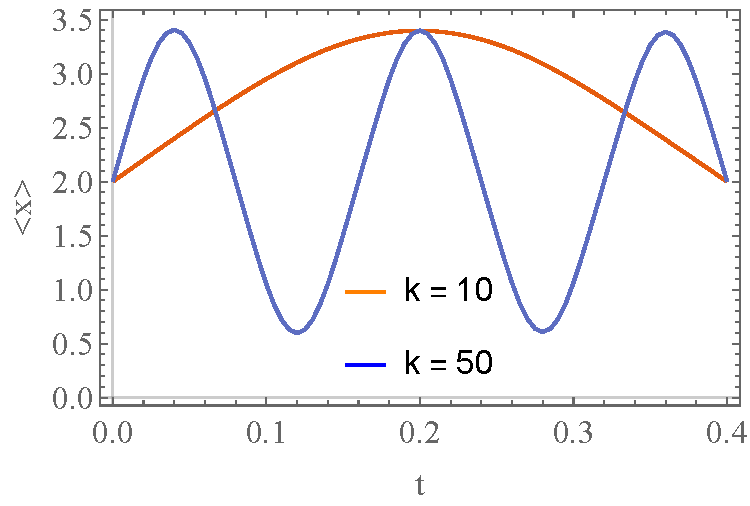
\includegraphics[scale=0.55]{img/rt_expect}
\caption{Valores de expectación de $x(t)$.}
\label{fig:expec}
\end{figure}

El tiempo de retorno es el tiempo en el que la partícula realiza dos choques con la pared y su valor de expectación vuelve a ser cero, es decir, si se grafica el tiempo de expectación respecto al tiempo, corresponde al tiempo en el que ocurre el tercer cero de la función.

Alternativamente, el tiempo de expectación clásico se puede calcular a través de l mecánica clásica y queda en términos de
\[
	T_{RCl} = L \sqrt{\frac{2M}{E}}.
\]

Si se compara el tiempo de retorno clásico con el tiempo de retorno cuántico que se obtiene a partir del método descrito anteriormente se obtienen los resultados que se muestran en la figura \ref{fig:tret}.

\begin{figure}[h!]
\begin{subfigure}{.5\textwidth}
	\centering
	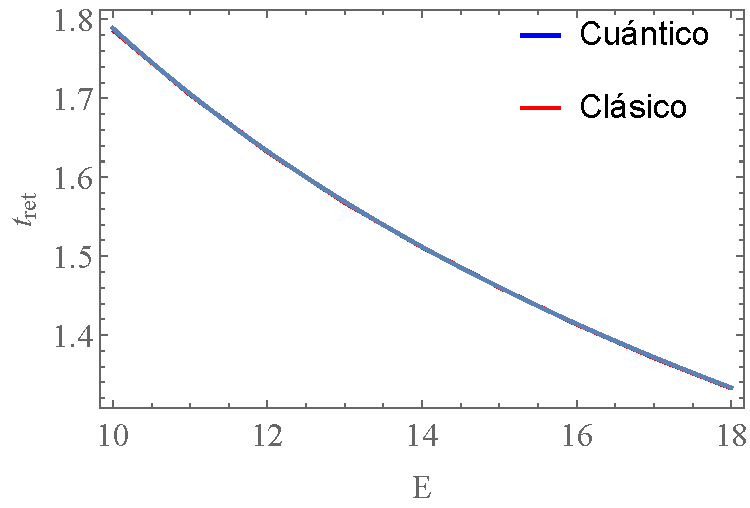
\includegraphics[scale=0.60]{img/le}
\end{subfigure}%
\begin{subfigure}{.5\textwidth}
	\centering
	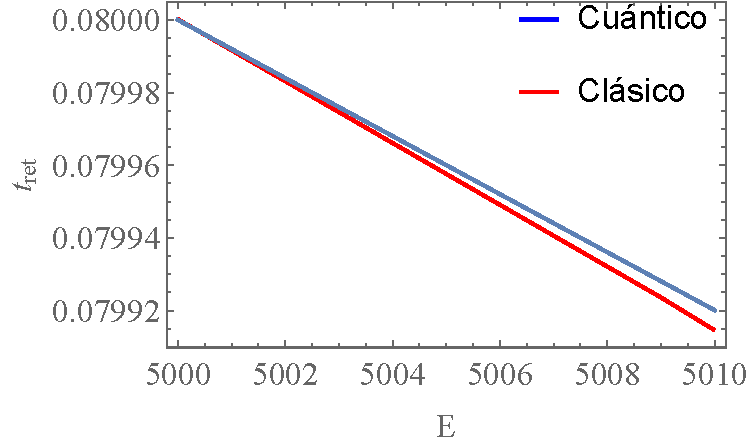
\includegraphics[scale=0.60]{img/he}
\end{subfigure}%
\caption{Comparación de tiempos de retorno.}
\label{fig:tret}
\end{figure}

En este resultado se observa que la discrepancia entre el tiempo de retorno clásico no es notable a bajas energías, pero conforme aumenta la energía la discrepancia se hace más evidente.

\section{Referencias}
\renewcommand*{\refname}{}
\begin{thebibliography}{100}

\bibitem{RT} \url{http://www.oberlin.edu/physics/dstyer/TeachQM/Revive.pdf}
 
\end{thebibliography}

\end{document}
